\renewcommand{\cache}[1]{\phantomchoix{#1}\hspace*{0.1mm}}

%%% utilisation des algorithmes
\usepackage{algorithm}
\usepackage{algorithmic}
\renewcommand{\algorithmicrequire} {\textbf{\textsc{Entrées:}}}
\renewcommand{\algorithmicensure}  {\textbf{\textsc{Sorties:}}}
\renewcommand{\algorithmicwhile}   {\textbf{tantque}}
\renewcommand{\algorithmicdo}      {\textbf{faire}}
\renewcommand{\algorithmicendwhile}{\textbf{fin tantque}}
\renewcommand{\algorithmicend}     {\textbf{fin}}
\renewcommand{\algorithmicif}      {\textbf{si}}
\renewcommand{\algorithmicendif}   {\textbf{finsi}}
\renewcommand{\algorithmicelse}    {\textbf{sinon}}
\renewcommand{\algorithmicthen}    {\textbf{alors}}
\renewcommand{\algorithmicfor}     {\textbf{pour}}
\renewcommand{\algorithmicforall}  {\textbf{pour tout}}
\renewcommand{\algorithmicdo}      {\textbf{faire}}
\renewcommand{\algorithmicendfor}  {\textbf{fin pour}}
\renewcommand{\algorithmicloop}    {\textbf{boucler}}
\renewcommand{\algorithmicendloop} {\textbf{fin boucle}}
\renewcommand{\algorithmicrepeat}  {\textbf{répéter}}
\renewcommand{\algorithmicuntil}   {\textbf{jusqu'à}}

\floatname{algorithm}{Algorithme}

\let\mylistof\listof
\renewcommand\listof[2]{\mylistof{algorithm}{Liste des algorithmes}}

% pour palier au problème de niveau des algos
\makeatletter
\providecommand*{\toclevel@algorithm}{0}
\makeatother

\begin{document}
\entetecoursinfo




\section{Introduction}

\subsection*{Le problème des sept ponts de Königsberg}

Le problème des sept ponts de Königsberg est connu pour être à l'origine de la théorie des graphes. Résolu par Leonhard Euler en 1735, ce problème se présente de la façon suivante~:


\begin{figure}[h]
    \begin{minipage}[c]{.32\linewidth}
        \centering
        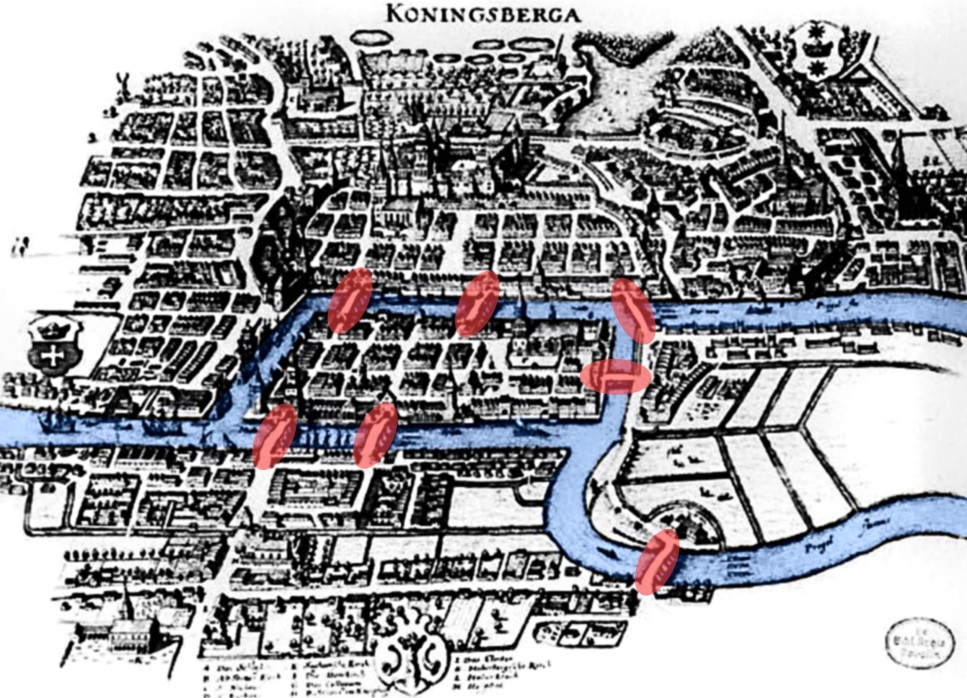
\includegraphics[height=0.7\textwidth]{images/ponts_rouge.jpg}
        \caption{Plan de la ville avec les ponts}
        \label{image1}
    \end{minipage}
    \hfill%
    \begin{minipage}[c]{.32\linewidth}
        \centering
        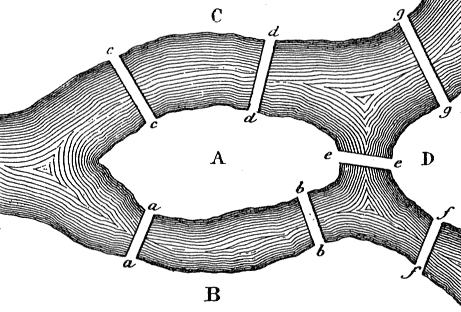
\includegraphics[height=0.7\textwidth]{images/lucas_ch2_fig1_50pc}
        \caption{Représentation schématisée vue du dessus}
    \end{minipage}
    \hfill%
    \begin{minipage}[c]{.32\linewidth}
        \centering
        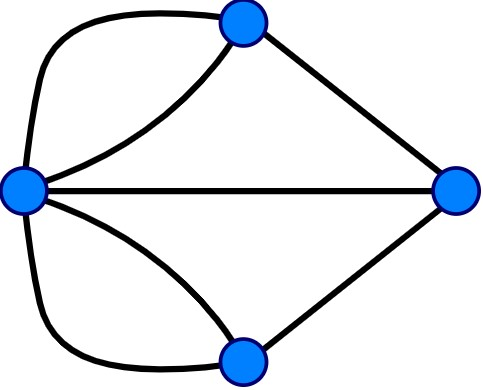
\includegraphics[height=0.7\textwidth]{images/ponts_graphe.jpg}
        \caption{Représentation sous forme de graphe}
    \end{minipage}
\end{figure}

La ville de Königsberg (aujourd'hui Kaliningrad) est construite autour de deux îles situées sur le fleuve Pregel et reliées entre elles par un pont. Six autres ponts relient les rives de la rivière à l'une ou l'autre des deux îles, comme représentés sur le plan de la figure \ref{image1}. Le problème consiste à déterminer s'il existe ou non une promenade dans les rues de Königsberg permettant, à partir d'un point de départ au choix, de passer une et une seule fois par chaque pont, et de revenir à son point de départ, étant entendu qu'on ne peut traverser le fleuve qu'en passant sur les ponts.\\

Les graphes, qui sont des diagrammes faits de cercles et de lignes, sont utilisés dans de nombreux domaines pour modéliser les relations entre différentes entités :
\begin{itemize}
\item liaisons mécaniques entre solides : le graphe de liaisons ;
\item liens sur les réseaux sociaux virtuels ou réels : relations entre personnes ;
\item les réseaux routiers : villes reliées par des routes ;
\item les réseaux de distributions de biens, d'énergie ;
\item en informatique, le routage et les relations entre des données : chaque sommet est une machine et les arêtes peuvent être une liaison physique ;
\item etc.
\end{itemize}
  

On remarquera que certaines relations peuvent être symétriques (en mécanique, si une pièce \textbf{1} est en liaison avec une pièce \textbf{2} alors \textbf{2} est en liaison avec \textbf{1}) ou asymétriques (sur une chaine youtube, A est abonné au compte de B ne veut pas dire que B est abonné à A).

\section{graphes et représentation}

\subsection{Définitions}

\begin{defi}
Un \textbf{graphe} (non orienté) $G=(S,A)$ est un couple composé :
\begin{itemize}
\item d'un ensemble $S$ de points appelés \textbf{sommets} ;
\item d'un ensemble $A$ d'\textbf{arêtes}, tels qu'à chaque arête $a_i$ sont associés deux éléments de $S$, appelés ses extrémités, et que nous noterons $\verb![!s_j,s_k\verb!]!$.
\end{itemize}
Les extrémités de l'arête $a_i$ sont dits \textbf{adjacents}.
\end{defi}

\vspace{-0.5cm}
Ces sommets sont aussi dits \textbf{voisins}. Pour les graphes \textbf{non orientés}, l'arête est une relation d'adjacence symétrique.\\
Les deux extrémités peuvent être distinctes ou confondues ; dans ce dernier cas, l'arête s'appelle une \textbf{boucle}.

\vspace{0.3cm}

\begin{minipage}[l]{0.5\linewidth}
\begin{center}
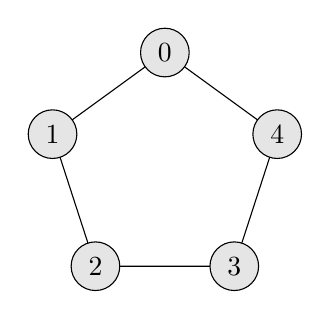
\begin{tikzpicture}[scale=1]
\tikzstyle{sommet}=[circle,draw,fill=gray!20]
\draw (90:1.5) node[sommet]{0}
-- (162:1.5) node[sommet]{1}
-- (234:1.5) node[sommet]{2}
-- (306:1.5) node[sommet]{3}
-- (378:1.5) node[sommet]{4}
-- cycle;
\end{tikzpicture}
\end{center}
\end{minipage}
\begin{minipage}[l]{0.5\linewidth}
Ce graphe $G=(S,A)$ est défini par :
\begin{itemize}
\item $S=\Cache{\{0,1,2,3,4\}}$
\item $A=\Cache{\{(0,1),(1,2),(2,3),(3,4),(4,0)\}}$
\end{itemize}
L'ordre des sommets
\end{minipage}
\Cache{dans les couples n'est pas important.}
\vspace{0.3cm}

Il existe de nombreux domaines où les graphes sont orientés (circuit électrique en courant continu, plan de ville avec sens interdit, ordonnancement d'une fabrication...)\\
Les arêtes des graphes \textbf{orientés} sont des \textbf{arcs} dont le sens va de l'extrémité initiale ou origine à l'extrémité terminale. Dans ce cas, on les représente sous forme de flèches. Les arcs sont des relations d'adjacence asymétriques.

\vspace{0.3cm}

\begin{minipage}[l]{0.5\linewidth}
\begin{center}
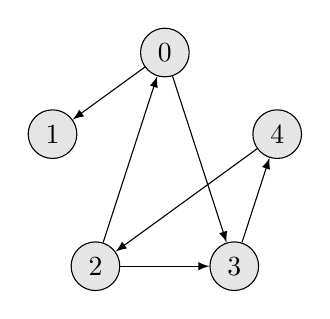
\begin{tikzpicture}[scale=1]
\tikzstyle{sommet}=[circle,draw,fill=gray!20]
\draw node[sommet](A0) at( 90:1.5) {0} ;
\draw node[sommet](A1) at (162:1.5){1} ;
\draw node[sommet](A2) at (234:1.5){2} ;
\draw node[sommet](A3) at (306:1.5){3} ;
\draw node[sommet](A4) at (378:1.5){4} ;
\draw[->,>=latex] (A0) -- (A1) ;
%\draw[->,>=latex] (A1) -- (A2) ;
\draw[->,>=latex] (A2) -- (A3)  ;
\draw[->,>=latex] (A3) -- (A4)  ;
%\draw[->,>=latex] (A4) -- (A0)  ;
\draw[->,>=latex] (A2) -- (A0)  ;
\draw[->,>=latex] (A0) -- (A3)  ;
%\draw[->,>=latex] (A3) -- (A1)  ;
%\draw[->,>=latex] (A4) -- (A1)  ;
\draw[->,>=latex] (A4) -- (A2)  ;
\end{tikzpicture}
\end{center}
\end{minipage}
\begin{minipage}[l]{0.5\linewidth}
Ce graphe $G=(S,A)$ est défini par :
\begin{itemize}
\item $S=\Cache{\{0,1,2,3,4\}}$
\item $A=\Cache{\{(0,1),(0,3),(4,2),(3,4),(2,3),(2,0)\}}$
\end{itemize}
L'ordre des sommets
\end{minipage}
\Cache{dans les couples est important.}
\newpage

\begin{defi}
\underline{Pour un graphe orienté}\\
Un \textbf{chemin} est une suite finie de sommets telle que deux sommets consécutifs soient adjacents.\\
La longueur d'un chemin est le nombre d'arcs constituant le chemin.\\
Un \textbf{circuit} est un chemin dont l'extrémité terminale est l'extrémité initiale et toutes ses arêtes sont distinctes.
\end{defi}

\begin{defi}
\underline{Pour un graphe non orienté}\\
Une \textbf{chaîne} est une suite finie de sommets telle que deux sommets consécutifs soient adjacents.\\
La longueur d'un chaîne est le nombre d'arêtes constituant la chaîne.\\
Un \textbf{cycle} est une chaîne dont l'extrémité terminale est l'extrémité initiale et toutes ses arêtes sont distinctes.
\end{defi}


\subsection{Représentation graphique}

Certains graphes jouent un rôle prépondérant dans la théorie des graphes. Par exemple,
un graphe à zéro arête est dit \textbf{vide} s'il ne comporte que des sommets, l'ensemble $A$ de ses arêtes est vide.

Un graphe simple (sans boucle ni arêtes parallèles) est dit \textbf{complet} si tous les sommets sont reliés entre eux.

Plusieurs représentations graphiques peuvent représenter le même graphe :

\begin{center}
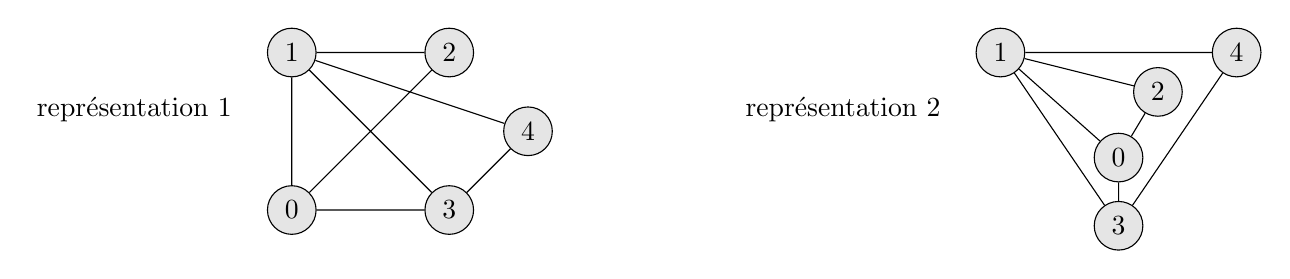
\begin{tikzpicture}[scale=1]
\tikzstyle{sommet}=[circle,draw,fill=gray!20]
\draw (-2,1) node[above] {représentation 1} ;
\node[sommet] (A0) at (0,0) {0};
\node[sommet] (A1) at (0,2) {1};
\node[sommet] (A2) at (2,2) {2};
\node[sommet] (A3) at (2,0) {3};
\node[sommet] (A4) at (3,1) {4};
\draw (7,1) node[above] {représentation 2} ;
\node[sommet] (B0) at (10.5,0.666) {0};
\node[sommet] (B1) at (9,2) {1};
\node[sommet] (B2) at (11,1.5) {2};
\node[sommet] (B3) at (10.5,-0.2) {3};
\node[sommet] (B4) at (12,2) {4};
\draw (A0) -- (A1) -- (A2) --(A0)--(A3)--(A4) --(A1)--(A3) ;
\draw (B0) -- (B1) -- (B2) --(B0) -- (B3) -- (B4) -- (B1) -- (B3);
\end{tikzpicture}
\end{center}

\begin{defi}
Un graphe est dit \textbf{connexe} si pour tout couple de sommets $(u, v)$ on trouve un chemin ou une chaîne entre $u$ et $v$.
\end{defi}

Un graphe peut être en plusieurs parties non reliées, ce graphe est non connexe.

\begin{center}
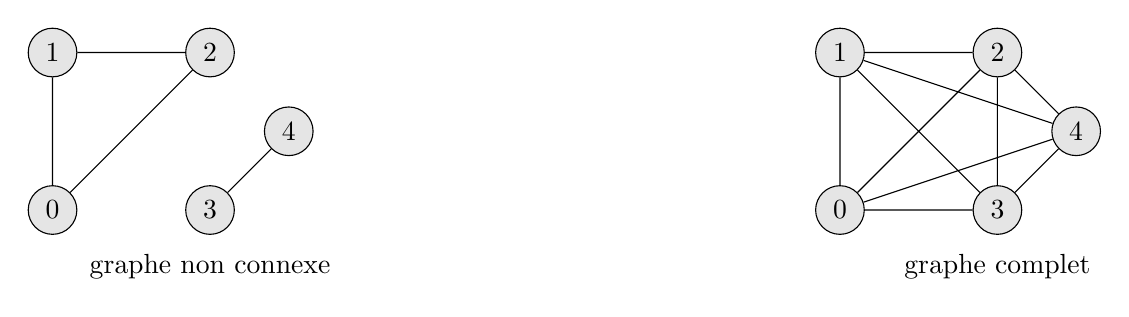
\begin{tikzpicture}[scale=1]
\tikzstyle{sommet}=[circle,draw,fill=gray!20]
\draw (2,-1) node[above] {graphe non connexe} ;
\node[sommet] (A0) at (0,0) {0};
\node[sommet] (A1) at (0,2) {1};
\node[sommet] (A2) at (2,2) {2};
\node[sommet] (A3) at (2,0) {3};
\node[sommet] (A4) at (3,1) {4};
\draw (12,-1) node[above] {graphe complet} ;
\node[sommet] (B0) at (10,0) {0};
\node[sommet] (B1) at (10,2) {1};
\node[sommet] (B2) at (12,2) {2};
\node[sommet] (B3) at (12,0) {3};
\node[sommet] (B4) at (13,1) {4};
\draw (A0) -- (A1) -- (A2) --(A0) ;
\draw (A4) -- (A3) ;
\draw (B0) -- (B1) -- (B2) -- (B3) -- (B4) -- (B0) -- (B2) -- (B4) -- (B1) -- (B3) -- (B0);
\end{tikzpicture}
\end{center}

\begin{defi}
Un \textbf{arbre} est un graphe connexe qui ne présente pas de cycle ou de circuit.
\end{defi}

\begin{center}
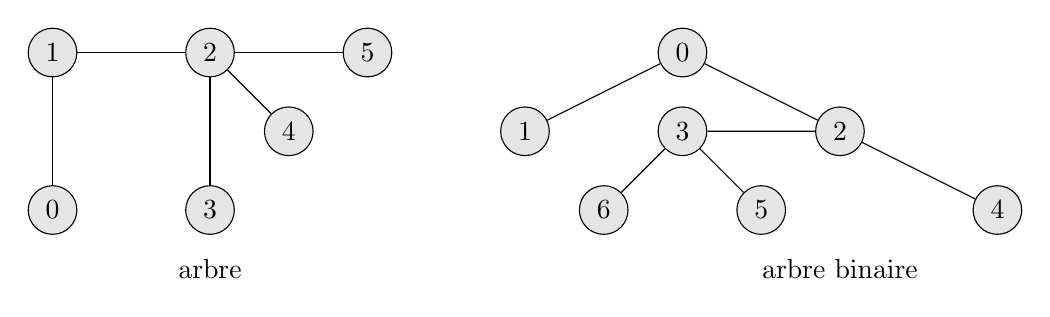
\begin{tikzpicture}[scale=1]
\tikzstyle{sommet}=[circle,draw,fill=gray!20]
\draw (2,-1) node[above] {arbre} ;
\node[sommet] (A0) at (0,0) {0};
\node[sommet] (A1) at (0,2) {1};
\node[sommet] (A2) at (2,2) {2};
\node[sommet] (A3) at (2,0) {3};
\node[sommet] (A4) at (3,1) {4};
\node[sommet] (A5) at (4,2) {5};
\draw (10,-1) node[above] {arbre binaire} ;
\node[sommet] (B1) at (6,1) {1};
\node[sommet] (B0) at (8,2) {0};
\node[sommet] (B2) at (10,1) {2};
\node[sommet] (B3) at (8,1) {3};
\node[sommet] (B4) at (12,0) {4};
\node[sommet] (B5) at (9,0) {5};
\node[sommet] (B6) at (7,0) {6};
\draw (A0) -- (A1) -- (A2) -- (A5) ;
\draw (A2) -- (A3) ;
\draw (A2) -- (A4) ;
\draw (B1) -- (B0) -- (B2) -- (B4);
\draw (B2) -- (B3) -- (B5);
\draw (B3) -- (B6);
\end{tikzpicture}
\end{center}


\subsection{Caractéristiques d'un graphe orienté ou non orienté}


\medskip
Si $(u,v)$ est un arc du graphe orienté $G=(S,A)$, on dit que l'arc $(u,v)$ est incident aux sommets $u$ et $v$ ou encore que l'arc $(u,v)$ quitte le sommet $u$ et arrive au sommet $v$.\\
On dit que $v$ est un \textbf{successeur} de $u$ et que $u$ est un \textbf{prédécesseur} de $v$.\\
Dans le cas non-orienté, on dit simplement que l'arête $\lbrace u, v \rbrace$ est incidente aux sommets $u$ et $v$.\\

\begin{defi}
On appelle \textbf{degré} du sommet $v$, noté $d(v)$, le nombre d'arêtes incidentes à ce sommet.\\
Le \textbf{degré d'un graphe} est le degré maximum de tous ses sommets.\\
L'\textbf{ordre} d'un graphe est le nombre $n$ de sommets du graphe.
\end{defi}

Si $m$ est le nombre d'arêtes, pour un graphe non orienté on aura la relation :

\Cache{
$$ \sum_{v \in V} d(v) = 2.m$$
}

\textit{Remarque :} On peut en déduire que le nombre de sommets de degré impair est forcément pair.

\smallskip
On désigne par \textbf{demi-degré extérieur} d'un sommet $v$ d'un graphe orienté, noté $d_+(v)$, le nombre d'arcs qui quittent $v$.\\
On désigne par \textbf{demi-degré intérieur} d'un sommet $v$ d'un graphe orienté, noté $d_-(v)$, le nombre d'arcs qui arrivent en $v$.\\
 
\Cache{$d(v) = d_+(v) + d_-(v)$}

\begin{minipage}[l]{0.5\linewidth}
\begin{center}
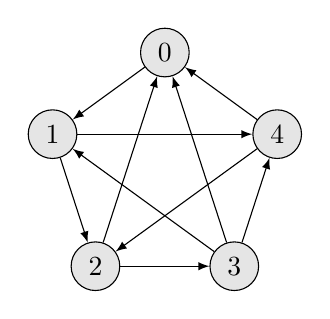
\begin{tikzpicture}[scale=1]
\tikzstyle{sommet}=[circle,draw,fill=gray!20]
\draw node[sommet](A0) at( 90:1.5) {0} ;
\draw node[sommet](A1) at (162:1.5){1} ;
\draw node[sommet](A2) at (234:1.5){2} ;
\draw node[sommet](A3) at (306:1.5){3} ;
\draw node[sommet](A4) at (378:1.5){4} ;
\draw[->,>=latex] (A0) -- (A1) ;
\draw[->,>=latex] (A1) -- (A2) ;
\draw[->,>=latex] (A2) -- (A3)  ;
\draw[->,>=latex] (A3) -- (A4)  ;
\draw[->,>=latex] (A4) -- (A0)  ;
\draw[->,>=latex] (A2) -- (A0)  ;
\draw[->,>=latex] (A3) -- (A0)  ;
\draw[->,>=latex] (A3) -- (A1)  ;
\draw[->,>=latex] (A1) -- (A4)  ;
\draw[->,>=latex] (A4) -- (A2)  ;
\end{tikzpicture}
\end{center}
\end{minipage}
\begin{minipage}[l]{0.5\linewidth}
Par exemple pour ce graphe on a: 
$$d_+(3) = \Cache{3}$$
$$d_-(3) = \Cache{1} $$
$$d(3)= \Cache{4}$$
\end{minipage}

\vspace{0.3cm}

Pour le graphe orienté représenté plus haut, nous avons comme chemin possible entre les sommets $3$ et $2$ :
$$\chi(3,2)= \Cache{{3,0,1,2}}$$

%\smallskip
%On appelle \textbf{distance} entre deux sommets la longueur de la plus petite chaîne les reliant.
%
%\smallskip
%On appelle \textbf{diamètre} d'un graphe la plus longue distance entre deux sommets.


Une chaîne est \textbf{élémentaire} si chaque sommet du graphe apparait au plus une fois.

\smallskip
Une chaîne est \textbf{simple} si chaque arête du graphe apparait au plus une fois.

%\begin{defi}
%Pour un graphe G ayant $m$ arêtes, $n$ sommets et $p$ composantes connexes, on définit le nombre cyclomatiques $\mu(G)$ du graphe par:
%$$\mu(G)= m - n + p $$
%Le nombre cyclomatique et positif et représente le nombre de cycles indépendants.
%\end{defi}

\begin{defi}
Une chaîne (resp. un chemin) est eulérienne si elle contient une fois et une seule chaque arête du graphe ; si la chaîne est un cycle, on l'appelle cycle eulérien.
\end{defi}


\section{Implémentation}

\subsection{Liste d'adjacence}

Une liste d'adjacence d'un graphe non orienté est une liste de listes G qui possède les propriétés suivantes~: 
\begin{itemize}
	\item elle est constituée de $n$ listes correspondant aux $n$ sommets du graphe ;
	\item la liste G\verb![!i\verb!]! contient tous les voisins de $i$. 
\end{itemize}

On a donc la représentation du graphe :

\begin{center}
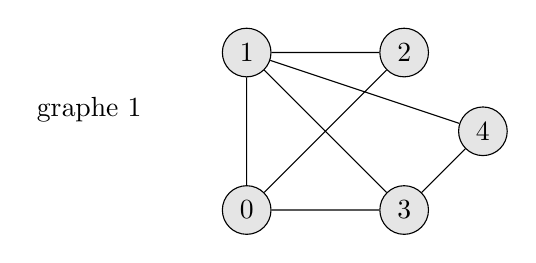
\begin{tikzpicture}[scale=1]
\tikzstyle{sommet}=[circle,draw,fill=gray!20]
\draw (-2,1) node[above] {graphe 1} ;
\node[sommet] (A0) at (0,0) {0};
\node[sommet] (A1) at (0,2) {1};
\node[sommet] (A2) at (2,2) {2};
\node[sommet] (A3) at (2,0) {3};
\node[sommet] (A4) at (3,1) {4};
\draw (A0) -- (A1) -- (A2) --(A0)--(A3)--(A4) --(A1)--(A3) ;
\end{tikzpicture}
\end{center}

\Cache{
\texttt{G1 = [[1,2,3],[0,2,3,4], [0,1], [0,1,4], [1,3]]}.}

Dans le cas d'un graphe orienté, la liste d'adjacence contient la liste des successeurs.

\subsection{Dictionnaire d'adjacence}

Un dictionnaire d'adjacence d'un graphe non-orienté est un dictionnaire $D$ de listes qui possède les propriétés suivantes :
\begin{itemize}
	\item il est constitué de $n$ listes correspondant aux $n$ sommets du graphe ;
	\item $D\verb![!s_i\verb!]!$ est une liste contenant tous les voisins de $s_i$. 
\end{itemize}

On a donc la représentation du graphe 1 :

\Cache{
\texttt{D1 = \{0:[1,2,3], 1:[0,2,3,4], 2:[0,1], 3:[0,1,4], 4:[1,3]\}}
}

L'avantage d'un dictionnaire d'adjacence est la possibilité de nommer les sommets. On peut l'adapter de la même manière que la liste par adjacence pour représenter un graphe orienté. 

\subsection{Matrice d'adjacence}

Une matrice d'adjacence d'un graphe non orienté est une matrice \texttt{M} qui possède les propriétés suivantes~:
\begin{itemize}
	\item elle est de taille $n \times n$, $n$ étant le nombre de sommets du graphe ;
	\item $M\verb![!i\verb!]!\verb![!j\verb!]!=1$ s'il y a une arête entre $s_i$ et  $s_j$ ; 
	\item $M\verb![!i\verb!]!\verb![!j\verb!]!=0$ s'il n'existe pas d'arête entre $s_i$ et $s_j$.
\end{itemize}

On a donc la représentation du graphe 1 :


\begin{Verbatim}
    M = [[0, 1, 1, 1, 0],
         [1, 0, 1, 1, 1],
         [1, 1, 0, 0, 0],
         [1, 1, 0, 0, 1],
         [0, 1, 0, 1, 0]]
\end{Verbatim}


On remarquera qu'un graphe non-orienté possède forcément une matrice d'adjacence symétrique.\\
Si le graphe présente une boucle sur le sommet $i$, alors la valeur $M\verb![!i\verb!]!\verb![!i\verb!]!=2$.\\

On peut remplacer les valeurs de la matrice par les booléens \texttt{True} et \texttt{False}.

\begin{Verbatim}
    M = [[False, True, True, True, False],
         [True, False, True, True, True],
         [True, True, False, False, False],
         [True, True, False, False, True],
         [False, True, False, True, False]]
\end{Verbatim}

On peut adapter cette matrice pour représenter un graphe orienté~: on remplace les arêtes $\{s_i, s_j\}$ par les arcs $(s_i, s_j)$. 

Cette matrice peut-être codée avec une liste de listes ou un tableau \texttt{numpy}.
%Mais elle peut aussi être codée grâce à un dictionnaire de dictionnaires possédant les propriétés suivantes~:
%\begin{itemize}
%	\item $M[s_i][s_j]=1$ s'il y a un arc d'extrémité initiale $s_i$ et d'extrémité terminale $s_j$~; 
%	\item $M[s_i][s_j]=0$ s'il n'existe pas un arc d'extrémité initiale $s_i$ et d'extrémité terminale $s_j$.
%\end{itemize}
%
%Cela permet, encore une fois, de faciliter la lecture en utilisant des noms pour les sommets, et pas seulement des indices compris dans l'intervalle $[ 0 ; \#S -1 ]$.
%
%On a donc la représentation du graphe de la :
%\begin{Verbatim}
%    d = {'a': {'a': 0, 'b': 1, 'c': 0, 'd': 0, 'e': 0}, 
%	     'b': {'a': 0, 'b': 0, 'c': 1, 'd': 1, 'e': 0}, 
%	     'c': {'a': 0, 'b': 0, 'c': 0, 'd': 1, 'e': 0}, 
%	     'd': {'a': 0, 'b': 1, 'c': 0, 'd': 0, 'e': 1}, 
%	     'e': {'a': 0, 'b': 0, 'c': 0, 'd': 0, 'e': 1}}
%\end{Verbatim}
%
%L'important avantage comparé aux simples listes et dictionnaires d'adjacence est de facilement s'adapter à l'ajout de pondérations sur les arcs ou les arêtes.




\section{Graphe pondéré}

On peut enrichir la notion de graphe en attribuant des poids aux arcs et aux arêtes. Concrètement, ces poids peuvent représenter des distances, des temps de parcours, des coûts de transport, des coûts de construction, etc.

\begin{figure}[hb]
	\begin{center}
		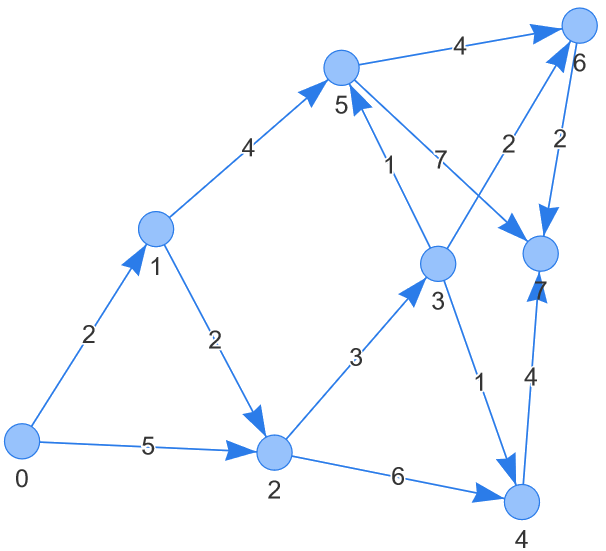
\includegraphics[width=0.35\linewidth]{images/oriente_pondere}
		\caption{Exemple de représentation d'un graphe orienté pondéré}
		\label{pondere}
	\end{center}
\end{figure}

\subsection{Vocabulaire}


\begin{defi}
Un arc pondéré est un couple (arc, poids).\\
Une arête pondérée est un couple (arête, poids).
\end{defi}

\begin{defi}
Un graphe orienté $G = (S,A)$ pondéré est un couple de sommets et d'arcs pondérés.\\
Un graphe non-orienté $G = (S,A)$ pondéré est un couple de sommets et d'arêtes pondérées.
\end{defi}

\subsection{Matrice de pondération}

Une matrice de pondération est une matrice d'adjacence adaptée~: 
\begin{itemize}
	\item $M\verb![!i\verb!]!\verb![!j\verb!]!= w$ s'il y a un arc de poids $w$ d'extrémité initiale $s_i$ et d'extrémité terminale $s_j$~; 
	\item $M\verb![!i\verb!]!\verb![!j\verb!]!=0$ (ou $M\verb![!i\verb!]!\verb![!j\verb!]!=\infty$) s'il n'existe pas un arc d'extrémité initiale $s_i$ et d'extrémité terminale $s_j$.
\end{itemize}


On a donc la représentation du graphe de la figure \ref{pondere} :

\begin{Verbatim}
    M = [[0, 2, 5, 0, 0, 0, 0, 0],
         [0, 0, 2, 0, 0, 4, 0, 0],
         [0, 0, 0, 3, 6, 0, 0, 0],
         [0, 0, 0, 0, 1, 0, 2, 0],
         [0, 0, 0, 0, 0, 0, 0, 4],
         [0, 0, 0, 1, 0, 0, 4, 7],
         [0, 0, 0, 0, 0, 0, 0, 2],
         [0, 0, 0, 0, 0, 0, 0, 0]]
\end{Verbatim}

Comme précédemment, on peut coder cette matrice avec un dictionnaire de dictionnaires afin de pouvoir utiliser des noms plus explicites au niveau des sommets.

On a donc la représentation du graphe de la figure \ref{pondere} :

\begin{Verbatim}
    D = {0: {0: 0, 1: 2, 2: 5, 3: 0, 4: 0, 5: 0, 6: 0, 7: 0}, 
         1: {0: 0, 1: 0, 2: 2, 3: 0, 4: 0, 5: 4, 6: 0, 7: 0}, 
         2: {0: 0, 1: 0, 2: 0, 3: 3, 4: 6, 5: 0, 6: 0, 7: 0}, 
         3: {0: 0, 1: 0, 2: 0, 3: 0, 4: 1, 5: 0, 6: 2, 7: 0}, 
         4: {0: 0, 1: 0, 2: 0, 3: 0, 4: 0, 5: 0, 6: 0, 7: 4}, 
         5: {0: 0, 1: 0, 2: 0, 3: 1, 4: 0, 5: 0, 6: 4, 7: 7}, 
         6: {0: 0, 1: 0, 2: 0, 3: 0, 4: 0, 5: 0, 6: 0, 7: 2}, 
         7: {0: 0, 1: 0, 2: 0, 3: 0, 4: 0, 5: 0, 6: 0, 7: 0}}
\end{Verbatim}

On peut l'adapter pour représenter un graphe non-orienté~: on remplace les arcs $(s_i, s_j)$ par les arêtes $\{s_i, s_j\}$. Comme précédemment, une matrice de pondération d'un graphe non-orienté est forcément symétrique.




%\newpage
%
%\Cache{
%On utilise sa notation binaire. \\
%Par exemple, $127=2^7-1=\dfrac{1-2^7}{1-2}=2^0+2^1+\dots+2^6$ donc sa représentation binaire est, avec $8$ bits, \uline{01111111}.
%}
%
%
%
%\begin{pythonshell}
%\invite 2.0**(60) + 1 - 2.0**(60)\\
%0.0
%\end{pythonshell}
%
%
%\begin{lstlisting}
%def nbsolutions(a,b,c):
%	Delta = b**2 - 4*a*c
%	if Delta == 0:
%		nb = 1
%	elif Delta > 0:
%		nb = 2
%	else:
%		nb  = 0
%	return(nb)
%\end{lstlisting}

\section{Applications}

\subsection{Exemple d'implémentation d'après un sujet de l'XENS 2015}
On souhaite stocker en mémoire une liste non-ordonnée d'au plus n entiers sans redondance (i.e. ou aucun entier n'apparaît
plusieurs fois). Nous utilisons un tableau 
liste de longueur $n+1$ tel que :
\begin{itemize}
\item liste\verb![!0\verb!]! contient le nombre d'éléments dans le tableau ;
\item liste\verb![!i\verb!]! contient le $i^{ème}$ élément de la liste non-ordonnée avec $1\leqslant i \leqslant liste\verb![!0\verb!]!$.
\end{itemize}
Nous disposons d'une fonction \texttt{creerListeVide(n:int)->list} qui permet de créer une liste pouvant contenir $n$ éléments.

\begin{pythonshell}
\invite creerListeVide(3)\\
\verb![!0,None,None,None\verb!]!
\end{pythonshell}

Nous disposons d'une fonction \texttt{estDansListe(liste:list,x)->bool} qui renvoie $True$ si l'élément $x$ est dans la liste et $False$ sinon.\\
La complexité de cette fonction est linéaire en fonction du nombre d'élément maximum que peut contenir la liste. 
Nous disposons aussi d'une fonction \texttt{ajouteDansListe(liste:list,x)} qui modifie la liste pour ajouter l'élément $x$ s'il n'est pas présent et ne fait rien sinon. La complexité est aussi linéaire du nombre d'élément maximum que peut contenir la liste.

\medskip
Un plan $P$ est défini par un ensemble de $n$ villes numérotées de $1$ à $n$ et un ensemble de $m$ routes (toutes à double sens)
reliant chacune deux villes. On dira que deux villes $x, y \in  n$ sont voisines lorsqu'elles sont reliées par une route, ce que l'on notera $(x, y)$. On appellera chemin de longueur $k-1$ toute suite de villes $\verb![!v_1, v_2 ... , v_k\verb!]!$. Un plan $P$ est alors un graphe dont les sommets sont les villes et les routes les arêtes.

\medskip
\begin{minipage}[c]{0.48\linewidth}
\textbf{Structure de données. } Nous représentons tout plan $P$ à $n$ villes par un tableau plan de $(n+1)$ tableaux où :
\begin{itemize}
\item plan\verb![!0\verb!]! contient un tableau de deux éléments où :
\begin{itemize}
\item[.] plan\verb![!0\verb!]!\verb![!0\verb!]! a pour valeur le nombres $n$ de villes;
\item[.] plan\verb![!0\verb!]!\verb![!1\verb!]! a pour valeur le nombres $m$ de routes.
\end{itemize}
\end{itemize}
\end{minipage}
\hfill%
\begin{minipage}[c]{0.48\linewidth}
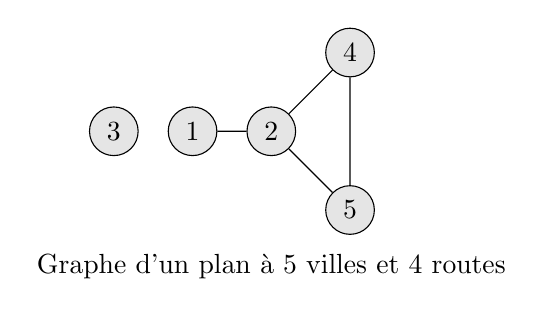
\begin{tikzpicture}[scale=1]
\tikzstyle{sommet}=[circle,draw,fill=gray!20]
\tikzstyle{arete}=[midway,fill=white]
\node[sommet] (S3) at (1,1) {3};
\node[sommet] (S1) at (2,1) {1};
\node[sommet] (S2) at (3,1) {2};
\node[sommet] (S4) at (4,2) {4};
\node[sommet] (S5) at (4,0) {5};
\draw (3,-1) node[above] {Graphe d'un plan à 5 villes et 4 routes} ;
\draw (S1) -- (S2) -- (S4)--(S5)--(S2) ; 
\end{tikzpicture}
\begin{lstlisting}
plan1= [[5,4] ,
         [1,2,None,None,None],
         [3,4,1,5,None],
         [0,None,None,None,None],
         [2,2,5,None,None],
         [2,4,2,None,None]]
\end{lstlisting}
\end{minipage}

\begin{itemize}
\item Pour toute ville $v \in n$, plan\verb![!v\verb!]! contient un tableau à $n$ éléments représentant 
la liste à au plus $(n-1)$ éléments des villes voisines de $v$ dans $P$ dans un ordre arbitraire en utilisant
la structure de liste sans redondance décrite plus haut. Ainsi :
\begin{itemize}
\item[.] plan\verb![!v\verb!]!\verb![!0\verb!]! a pour valeur le nombre de villes voisines de $v$ ;
\item[.] plan\verb![!v\verb!]!\verb![!1\verb!]! , ... ,n\verb![!v\verb!]!\verb![!n\verb![!v\verb!]!\verb![!0\verb!]!\verb!]! sont les indices des villes voisines de $v$
\end{itemize}
\end{itemize}

\medskip
\textbf{Question 1} : Représenter sous forme de tableaux les deux plans suivant :
\begin{center}
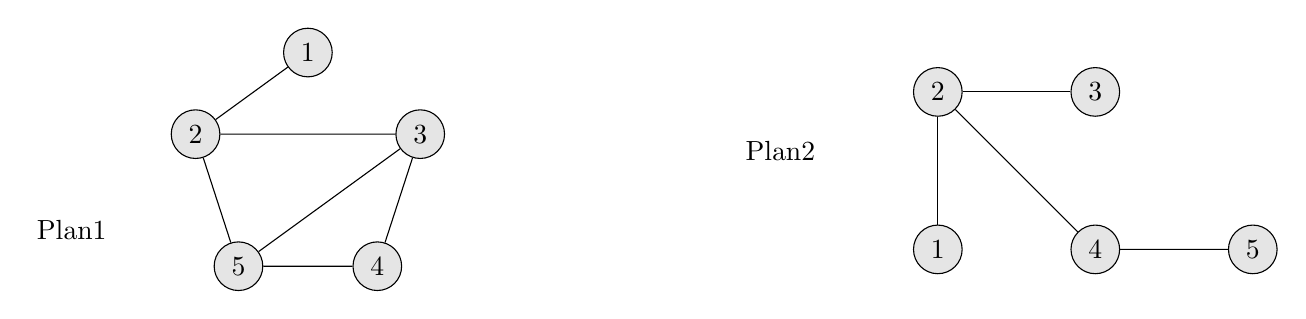
\begin{tikzpicture}[scale=1]
\tikzstyle{sommet}=[circle,draw,fill=gray!20]
\tikzstyle{arete}=[midway,fill=white]
\node[sommet] (A1) at ( 90:1.5) {1};
\node[sommet] (A2) at (162:1.5) {2};
\node[sommet] (A5) at (234:1.5) {5};
\node[sommet] (A4) at (306:1.5) {4};
\node[sommet] (A3) at ( 18:1.5) {3};
\draw (A1)--(A2)--(A3) -- (A4) -- (A5) --(A2);
\draw (A5)--(A3);
\draw (-3,-1) node[above] {Plan1} ;
\node[sommet] (B1) at (8,-1) {1};
\node[sommet] (B2) at (8,1) {2};
\node[sommet] (B3) at (10,1) {3};
\node[sommet] (B4) at (10,-1) {4};
\node[sommet] (B5) at (12,-1) {5};
\draw (6,0) node[above] {Plan2} ;
\draw (B1) -- (B2) -- (B3) ;
\draw (B2) -- (B4) -- (B5) ; 
\end{tikzpicture}
\end{center}


\textbf{Question 2} \'Ecrire une fonction \texttt{creerPlanSansRoute(n:int)} qui crée, remplit et renvoie le tableau de tableaux correspondant au plan à $n$ villes n'ayant aucune route.


\textbf{Question 3} \'Ecrire une fonction \texttt{estVoisine(plan,x,y)} qui renvoie $True$ si les villes $x$ et $y$ sont voisines dans le plan codé
par le tableau de tableaux plan et renvoie $False$ sinon.


\textbf{Question 4} \'Ecrire une procédure \texttt{ajouteRoute(plan,x,y)} qui modifie le tableau de tableaux plan pour ajouter une route 
entre les villes $x$ et $y$ si elle n'était pas déjà présente et ne fait rien sinon. On prendra garde à bien mettre à jour
toutes les cases concernées dans le tableau de tableaux plan. Y a-t-il un risque de dépassement de la capacité des listes ?


\textbf{Question 5} \'Ecrire une procédure \texttt{afficheToutesLesRoutes(plan)} qui affiche à l'écran la liste des routes du plan codé par le tableau de tableaux plan
où chaque route n'apparaît qu'une seule fois. Par exemple, pour le graphe codé par le tableau de tableaux de la présentation votre procédure pourra afficher :
\begin{lstlisting}
Ce plan contient 4 route(s) : (1-2) (2-4) (2-3) (4-5)
\end{lstlisting}
Quelle est la complexité de votre procédure ?

\subsection{Graphe d'intervalles : Énigme de Claude BERGE}
A l'époque, le Duc de Densmore avait été tué par l'explosion d'une bombe artisanale, qui avait également détruit le château de Densmore
où il s'était retiré. Les journaux d'alors relataient que le testament, détruit lui aussi par l'explosion, avait tout pour
déplaire à l'une de ses huit ex-femmes. Or, avant sa mort, le Duc les avait toutes invitées à passer quelques jours dans sa retraite écossaise.

Les suspects sont donc ces huit femmes présentes sur l'île au moment des faits. Chacune n'y ayant effectué qu'un seul
séjour. L'une d'entre elles a dû se cacher à un moment propice pour aller préparer et poser la bombe.

Les faits étant assez anciens, les suspects se souviennent des personnes qu'elles ont croisées, mais pas dans quel ordre. Voici les témoignages :

\begin{itemize}
\item Ann a déclaré y avoir rencontré Betty, Cynthia, Emily, Felicia et Georgia ;
\item Betty a déclaré y avoir rencontré Ann, Cynthia et Helen ;
\item Cynthia a déclaré y avoir rencontré Ann, Betty, Diana, Émily et Helen;
\item Diana a déclaré y avoir rencontré Cynthia et Emily ;
\item Emily a déclaré y avoir rencontré Ann, Cynthia, Diana et Felicia ;
\item Felicia a déclaré y avoir rencontré Ann et Emily;
\item Georgia a déclaré y avoir rencontré Ann et Helen ;
\item Helen a déclaré y avoir rencontré Betty, Cynthia et Georgia.
\end{itemize}

\medskip 
Précision supplémentaire, personne d'autre n'est venu sur l'île. Par ailleurs si deux femmes ne se sont pas vues,
c'est soit qu'elles n'étaient pas l'île en même temps, soit que l'une d'entre elles était cachée dans le labyrinthe et préparait la bombe artisanale ... 

\medskip
L'inspecteur qui vous a précédé sur l'affaire a constaté que les témoignages concordaient et avaient conclue
à la culpabilité du majordome mort dans l'explosion avec le duc. Mais ce n'est pas le cas. Pouvez-vous trouver le coupable ?


\vfill
\textbf{Références :}\\
T. Kovaltchouk, \textit{Informatique Commune PCSI}, Reims\\
UPSTI, \textit{Informatique Commune}



\newpage
\renewcommand{\contentsname}{Plan du cours}
\tableofcontents


\end{document}
